\chapter{Tribal NeuroSim: Game Logic and Neural Decision-Making}

\section{Neural Decision-Making and Cluster Priors}

Every simulated tribe carries a neural network whose architecture follows the NEAT (\textit{NeuroEvolution of Augmenting Topologies}) paradigm \cite{stanleymiikkulainen2002}. The system \textit{does not apply backpropagation}: a tribe receives no training signal from real League of Legends matches. Instead, fitness is derived from the outcome of the simulation process --- survival time, territory acquired, population size, and polity tier achieved --- and is evaluated every thousand ticks \cite{holland1992}.

At initialisation, each tribe receives cluster-level performance metrics derived from real match history as its initial genome sequence: \textbf{A\_combat}, \textbf{A\_resource}, \textbf{A\_map\_objective}, \textbf{A\_risk}, \textbf{A\_team}. During initialisation, each tribe is assigned a \textit{Genome::new(11,~7)} structure with 11 input nodes, 7 output nodes, and 84 initial connections.

\section{The 11 Input Signals and 7 Output Drives}

Each tick, inference is run from the genome: the neural network reads 11 input signals and returns 7 output drives. Some inputs reflect the tribe's current state (food, population, danger); others are the performance profile inherited from the cluster, which mutates slowly at generational checkpoints. The outputs directly modulate the tribe's behavioural decisions: initiating war, expanding, forming alliances, or retreating.

\begin{table}[h]
  \centering
  \caption{The 11 input signals of the neural network.}
  \label{tab:neurosim-inputs}
  \begin{tabular}{|c|l|l|l|}
    \hline
    \textbf{Index} & \textbf{Variable name} & \textbf{Description} & \textbf{Nature} \\
    \hline
    0 & \textit{food\_ratio}         & Food stock / population                    & Dynamic \\
    1 & \textit{pop\_ratio}          & Population / maximum capacity               & Dynamic \\
    2 & \textit{territory}           & Claimed tiles / 100                         & Dynamic \\
    3 & \textit{feed\_risk}          & Starvation proximity (1{,}0 = critical)    & Dynamic \\
    4 & \textit{a\_combat}           & Combat performance artifact                  & Invariant* \\
    5 & \textit{a\_resource}         & Resource/economy artifact                    & Invariant* \\
    6 & \textit{a\_map\_objective}   & Objective control artifact                   & Invariant* \\
    7 & \textit{a\_team}             & Team coordination artifact                   & Invariant* \\
    8 & \textit{nearest\_enemy}      & Hex distance to nearest enemy               & Dynamic \\
    9 & \textit{nearest\_ally}       & Hex distance to nearest ally                & Dynamic \\
   10 & \textit{a\_risk}             & Risk tolerance artifact                      & Invariant* \\
    \hline
  \end{tabular}
  \begin{flushleft}
    \small{* Updated only at generational checkpoints (every 1000 ticks) via mutation.}
  \end{flushleft}
\end{table}

\begin{table}[h]
  \centering
  \caption{The 7 output drives and their effect on tribe behaviour.}
  \label{tab:neurosim-outputs}
  \begin{tabular}{|l|l|l|}
    \hline
    \textbf{Variable name} & \textbf{Behavioural effect} & \textbf{Activation threshold} \\
    \hline
    \textit{aggression}      & Modulates war-initiation probability            & $> 0{,}45$ \\
    \textit{resource\_drive} & Territory expansion priority                     & $> 0{,}25$ \\
    \textit{goal\_drive}     & Alliance initiation, polity advancement          & $> 0{,}55$ / $> 0{,}50$ \\
    \textit{migration\_drive}& Triggers migration (from \textit{Settling} state) & $> 0{,}55$ \\
    \textit{raid\_drive}     & Opportunistic war against weaker neighbour      & $> 0{,}35$ \\
    \textit{isolation}       & Rejection of alliance offers                     & $> 0{,}75$ \\
    \textit{expansion\_speed}& Tile-claim speed (cooldown modification)         & Continuous \\
    \hline
  \end{tabular}
\end{table}

\section{Fitness, Mutation, and Lineage Inheritance}

Fitness consists of five components: \textit{survival\_ticks}, \textit{territory}, \textit{population}, \textit{polity\_tier}, and \textit{war\_record}. Mutation occurs every 1000 ticks. The base mutation rate is $\mu_0 = 0{,}05$; this is differentiated by fitness rank:

\begin{equation}
\mu_i =
\begin{cases}
2\mu_0 & \text{if } r_i \leq 0{,}20 \text{ (bottom 20\%)} \\
\mu_0  & \text{if } 0{,}20 < r_i < 0{,}80 \\
\tfrac{1}{2}\mu_0 & \text{if } r_i \geq 0{,}80 \text{ (top 20\%)}
\end{cases}
\end{equation}

where $r_i \in [0,1]$ is the relative fitness rank of tribe $i$ in the population.

Fusion conditions for both parties: \textit{goal\_drive}~$> 0{,}55$, neither is in an \textit{AtWar} state, and \textit{isolation}~$< 0{,}75$. The heir genome from a fusion is a fitness-weighted blend: \textit{Genome::inherit\_from(parent\_a, parent\_b, fitness\_a, fitness\_b)}.

Output activity and fitness-differentiation data from the F2 early run (599 tribes, Flexset, 1200 ticks) and the liveness-fix details can be found in chapter 14 of the extended version \cite{premadegraph-full}.

\begin{figure}[H]
\centering
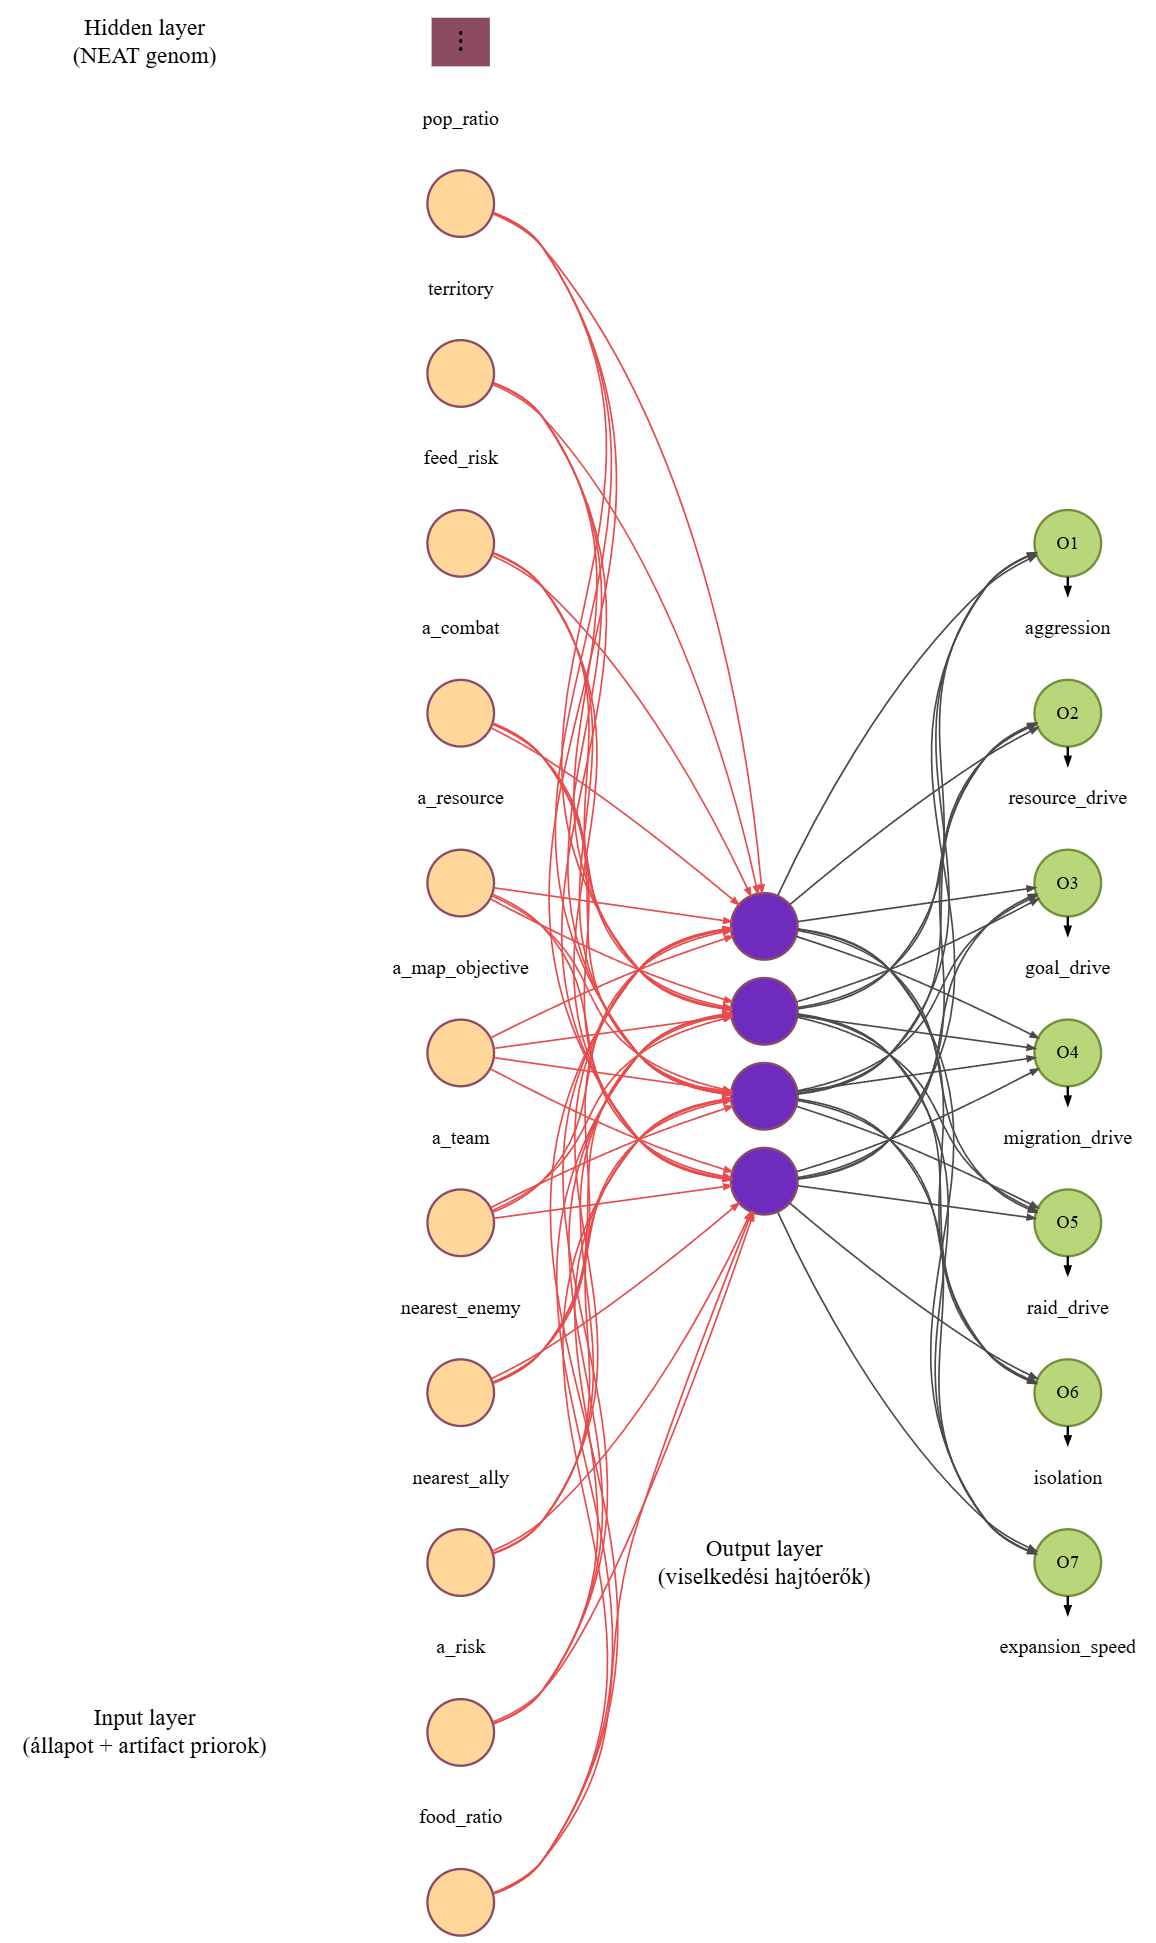
\includegraphics[width=0.95\textwidth,keepaspectratio]{assets/diagrams/genome_graph.png}
\caption{The genome graph: visualisation of the initial genome sequence built from PremadeGraph cluster-level performance metrics. The five axes (\textit{A\_combat}, \textit{A\_resource}, \textit{A\_map\_objective}, \textit{A\_risk}, \textit{A\_team}) form the invariant input signals of the neural network.}
\label{fig:genome-graph}
\end{figure}
